\chapter{Trajectory tracking via LQR}
\section{Dynamics Linearization and LQR Design}
% - Explain how dynamics are linearized around the trajectory (x_gen, u_gen).
In this task, the robot dynamics are linearized around the trajectory $(x^{\text{gen}}, u^{\text{gen}})$ computed in Task 2. Using the linearized model, the LQR algorithm is applied to design an optimal feedback controller for tracking the reference trajectory. The objective is to solve the following Linear-Quadratic (LQ) problem:

\[
\min_{\Delta x_1, \ldots, \Delta x_T, \atop \Delta u_0, \ldots, \Delta u_{T-1}} \quad
\sum_{t=0}^{T-1} \Delta x_t^\top Q_t^{\text{reg}} \Delta x_t + \Delta x_t^\top R_t^{\text{reg}} \Delta u_t + \Delta x_T^\top Q_T^{\text{reg}} \Delta x_T
\]



Subject to:  
\[
\Delta x_{t+1} = A_t^{\text{gen}} \Delta x_t + B_t^{\text{gen}} \Delta u_t, \quad t = 0, \ldots, T-1
\]  
\[
x_0 = 0
\]

Here, $\Delta x_t = x_t - x_t^{\text{gen}}$, where $A_t^{\text{gen}}$ and $B_t^{\text{gen}}$ are the matrices obtained by linearizing the nonlinear system dynamics around the reference trajectory $(x_{\text{gen}}, u_{\text{gen}})$. The cost matrices $Q_{\text{reg}}$ and $R_{\text{reg}}$ are tuning parameters that need to be defined during the regulator's setup. These matrices balance the trade-off between state deviations and control effort. In task 3 the behavior of the cost matrices is the following:

\begin{figure}[htb]
    \centering
    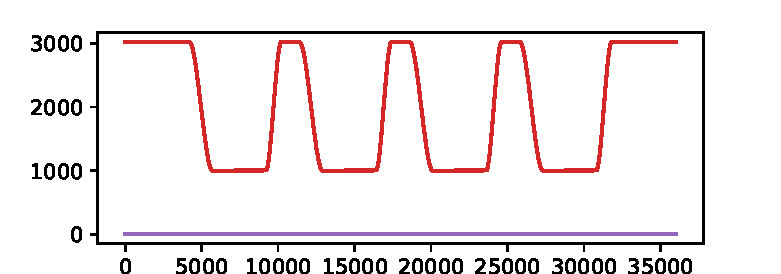
\includegraphics[width=0.8\linewidth]{img/3-task3/evolution_cost_task3.pdf}
    \caption{Evolution of cost matrices.}
    \label{fig:dtheta2-evolution}
\end{figure}

\newpage

To compute the feedback gain, the discrete Riccati equation is solved backward in time. Starting with $P_T = Q_T^{\text{reg}}$, compute recursively for $t = T-1, \ldots, 0$:
\[
P_t^{\text{reg}} = Q_t^{\text{reg}} + A_t^{\text{gen}, \top} P_{t+1}^{\text{reg}} A_t^{\text{gen}} \]
\[- \left( A_t^{\text{gen}, \top} P_{t+1}^{\text{reg}} B_t^{\text{gen}} \right) \left( R_t^{\text{reg}} + B_t^{\text{gen}, \top} P_{t+1}^{\text{reg}} B_t^{\text{gen}} \right)^{-1} \left( B_t^{\text{gen}, \top} P_{t+1}^{\text{reg}} A_t^{\text{gen}} \right)
\]


Using the results from the Riccati equation, the feedback gain $K_t^{\text{reg}}$ is calculated for all $t = 0, \ldots, T-1$:

\[
K_t^{\text{reg}} = -(R_t^{\text{reg}} + B_t^{\text{gen}, \top} P_{t+1} B_t^{\text{gen}})^{-1} 
(B_t^{\text{gen}, \top} P_{t+1} A_t^{\text{gen}})
\]
The LQR algorithm computes the control inputs in a feedback form, ensuring robustness. At each time step, the input is computed as a function of the deviation of the state from the reference trajectory:

\[
u_t = u_t^{\text{gen}} + K_t^{\text{reg}}(x_t - x_t^{\text{gen}})
\]

The system evolves according to:
\[
x_{t+1} = f_t(x_t, u_t), \quad t = 0, 1, \ldots
\]

To evaluate the tracking performance, the system should be tested with a perturbed initial condition, like an initial state that deviates from $x_0^{\text{gen}}$. The feedback controller should be able to compensate for this offset and guide the system back towards the reference trajectory, minimizing the tracking error over time.

% - Provide the linearized state-space equations.
% - Define the cost function and matrices Q, R, and \( Q_T \).
% - Explain how the LQR gain is computed (e.g., Riccati equations).
% - Discuss the rationale for matrix tuning.
\newpage
\section{Performance Analysis and Plots}
In Task 3, to test the tracking performance, a perturbed initial condition is considered, with a state perturbation percentage.

\begin{table}[h!]
\centering
\begin{tabular}{|c|c|}
\hline
\textbf{Case} & \textbf{State Perturbation Percentage} \\ \hline
Case 1        & 0.02                                   \\ \hline
Case 2        & 0.05                                   \\ \hline
Case 3        & -0.1                                   \\ \hline
\end{tabular}
\caption{Perturbation values for different cases}
\label{tab:perturbation_cases}
\end{table}

\begin{figure}[htb]
    \centering
    % First 3 images on the first page
    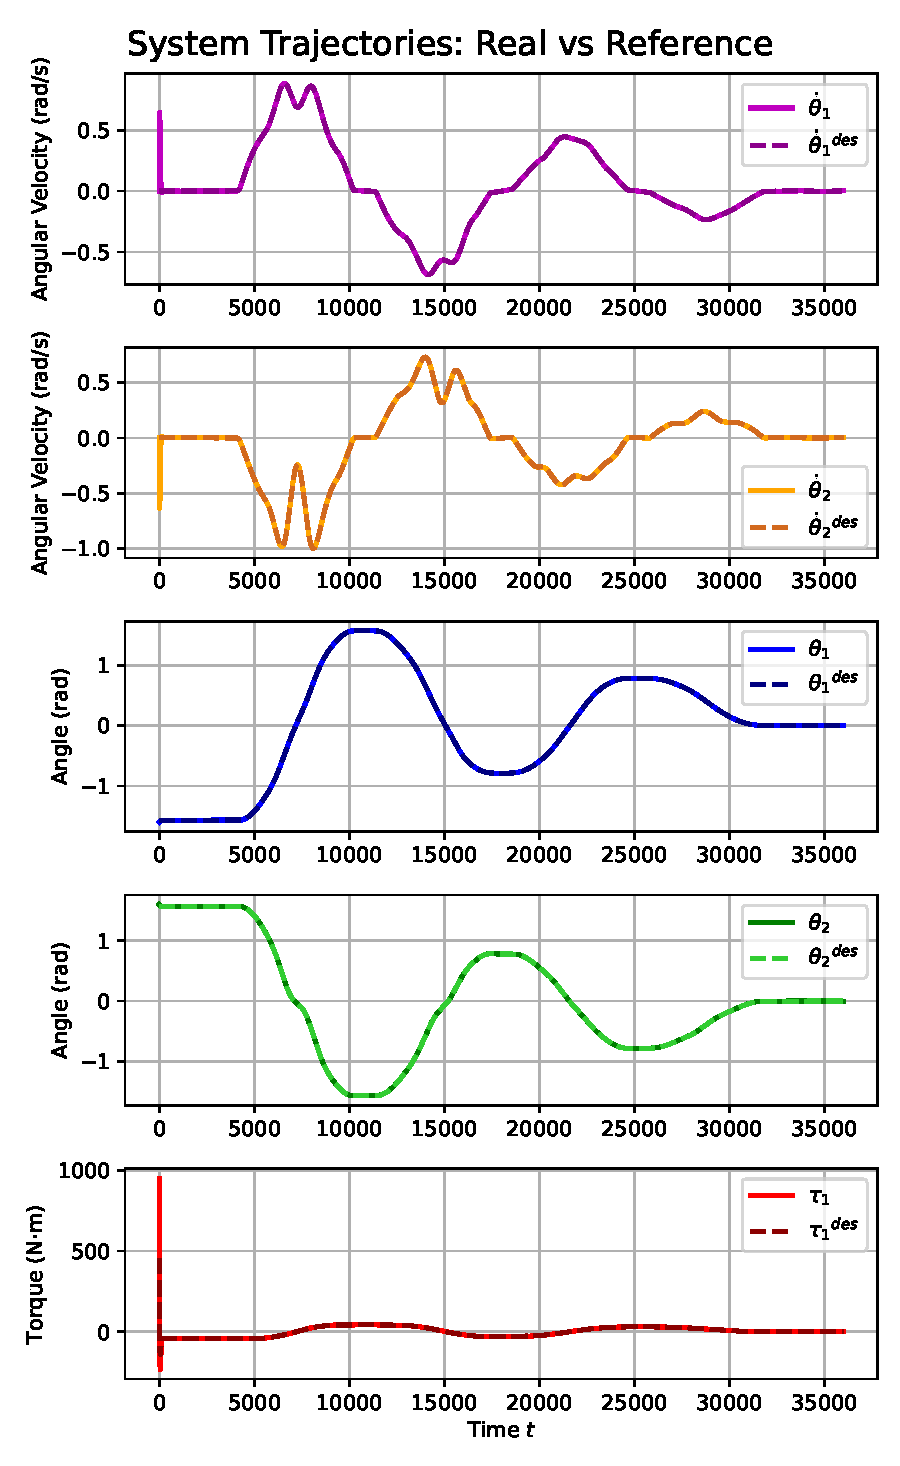
\includegraphics[width=1\linewidth]{img/3-task3/LQR1.pdf}
    \caption{Trajectories case 1}
    \label{fig:dtheta1-evolution}
\end{figure}

\begin{figure}[htb]
    \centering
    % First 3 images on the first page
    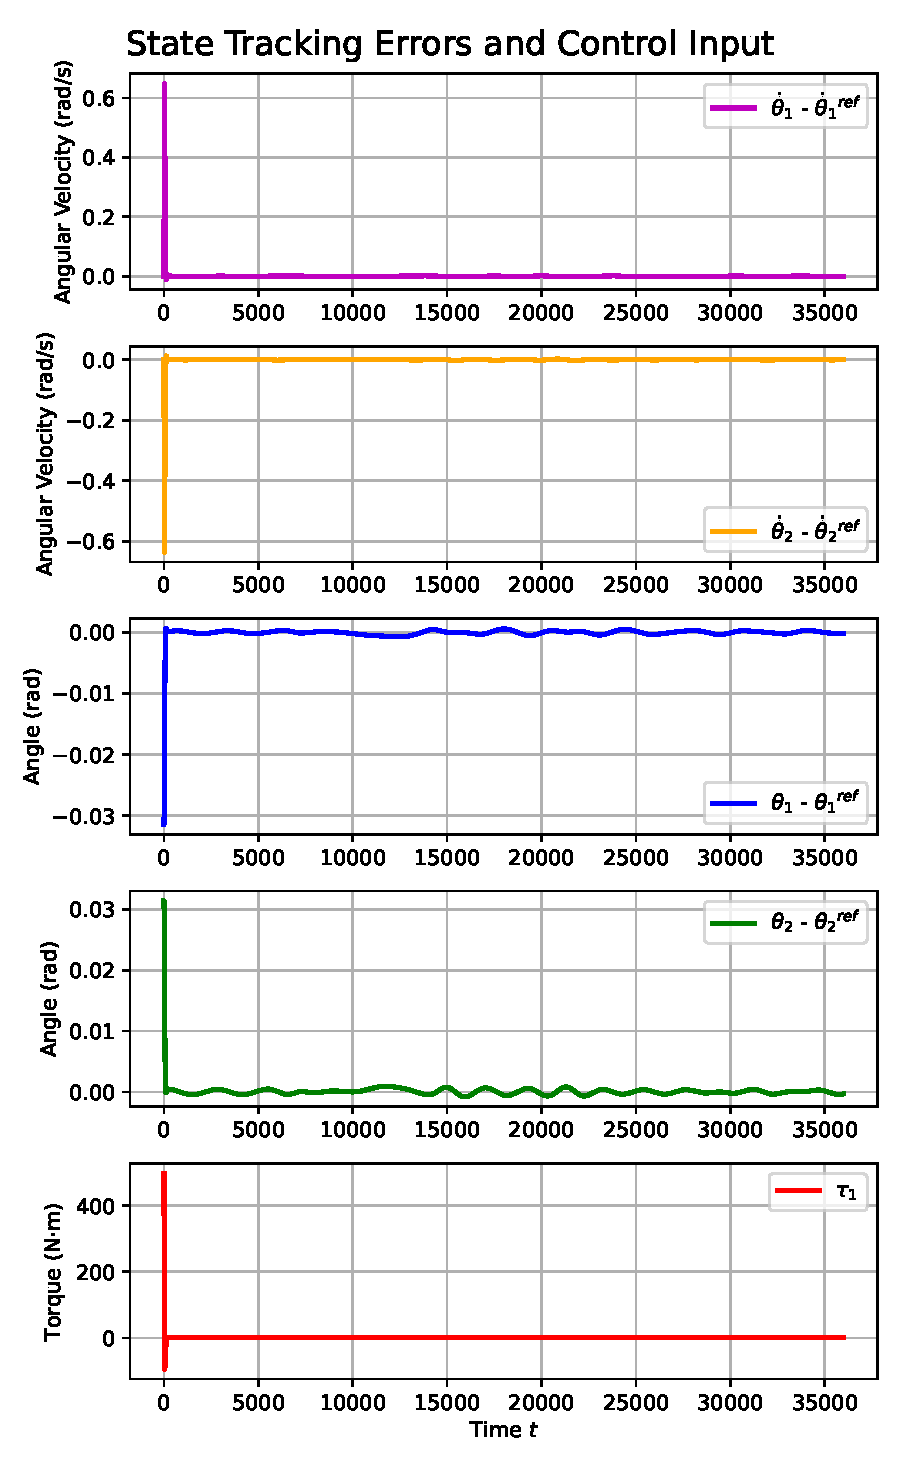
\includegraphics[width=1\linewidth]{img/3-task3/LQR1_errors.pdf}
    \caption{Tracking errors case 1}
    \label{fig:dtheta1-evolution}
\end{figure}

\begin{figure}[htb]
    \centering
    % First 3 images on the first page
    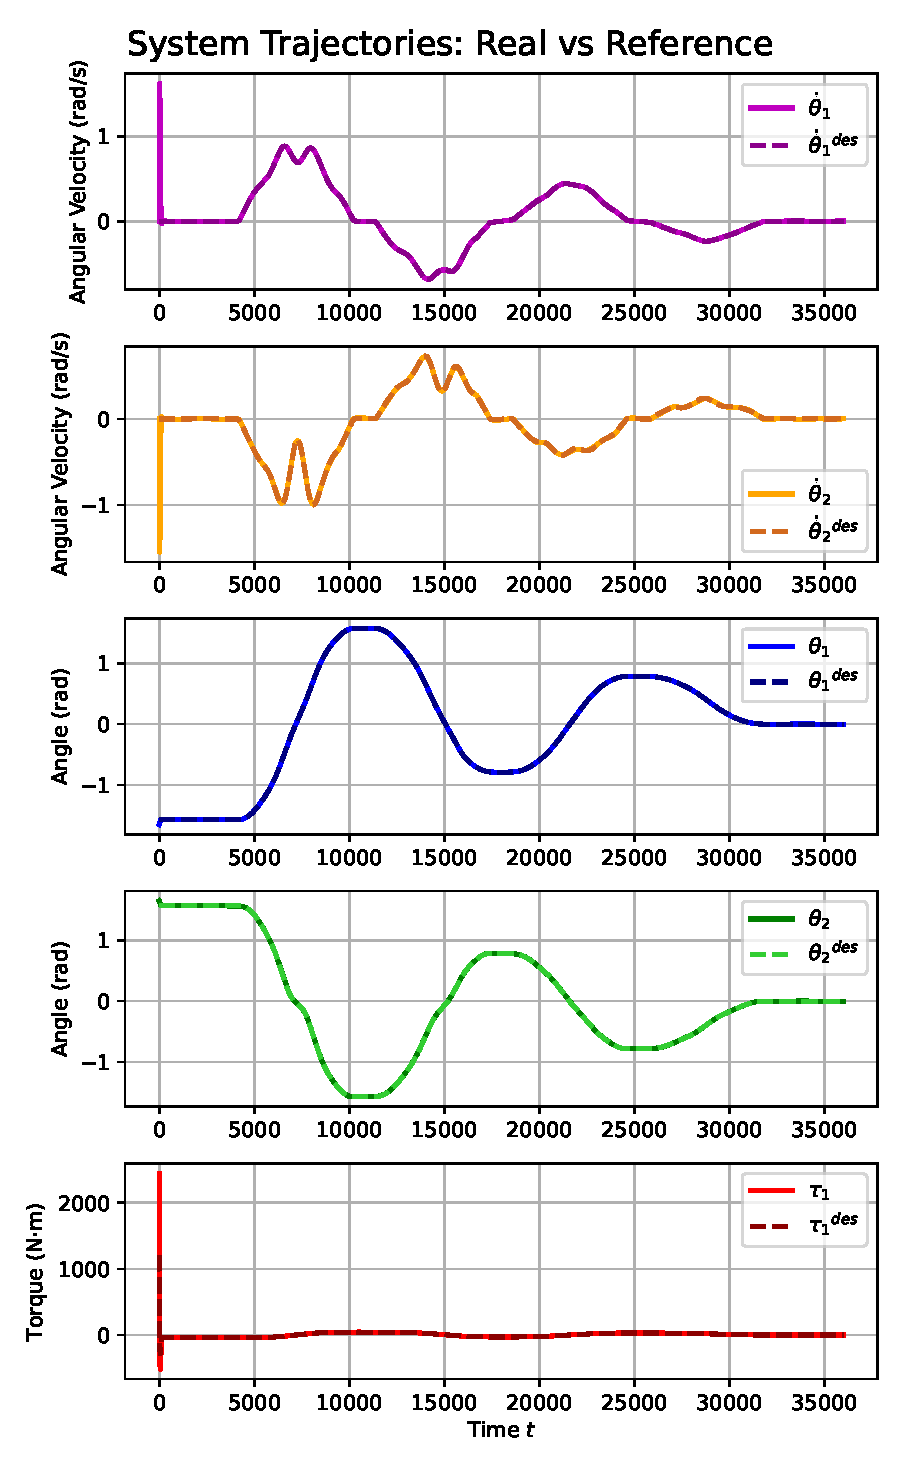
\includegraphics[width=1\linewidth]{img/3-task3/LQR2.pdf}
    \caption{Trajectories case 2}
    \label{fig:dtheta1-evolution}
\end{figure}

\begin{figure}[htb]
    \centering
    % First 3 images on the first page
    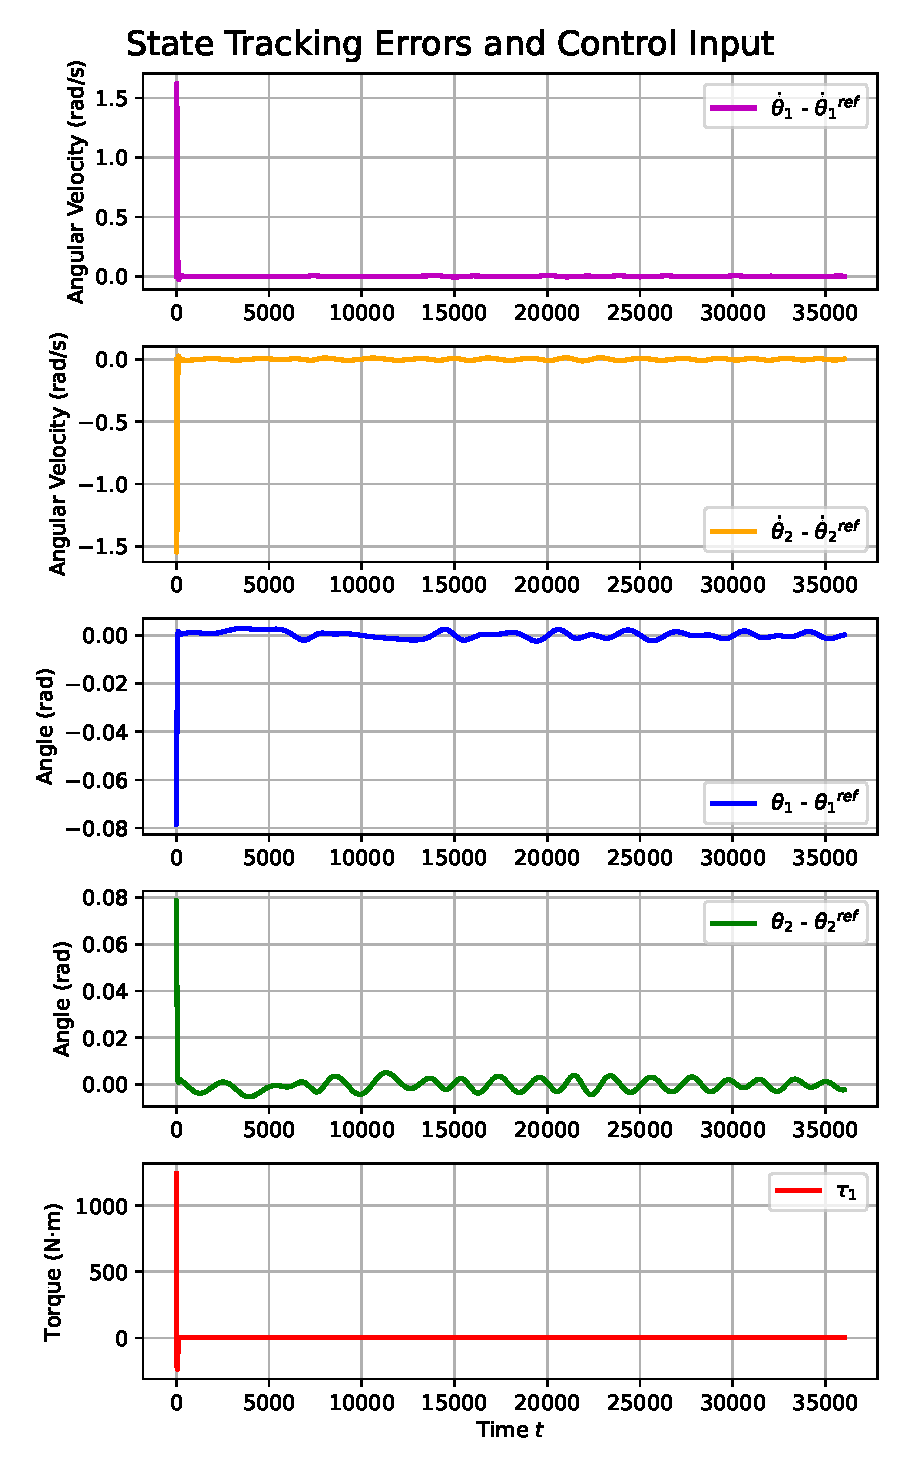
\includegraphics[width=1\linewidth]{img/3-task3/LQR2_errors.pdf}
    \caption{Tracking errors case 2}
    \label{fig:dtheta1-evolution}
\end{figure}

\begin{figure}[htb]
    \centering
    % First 3 images on the first page
    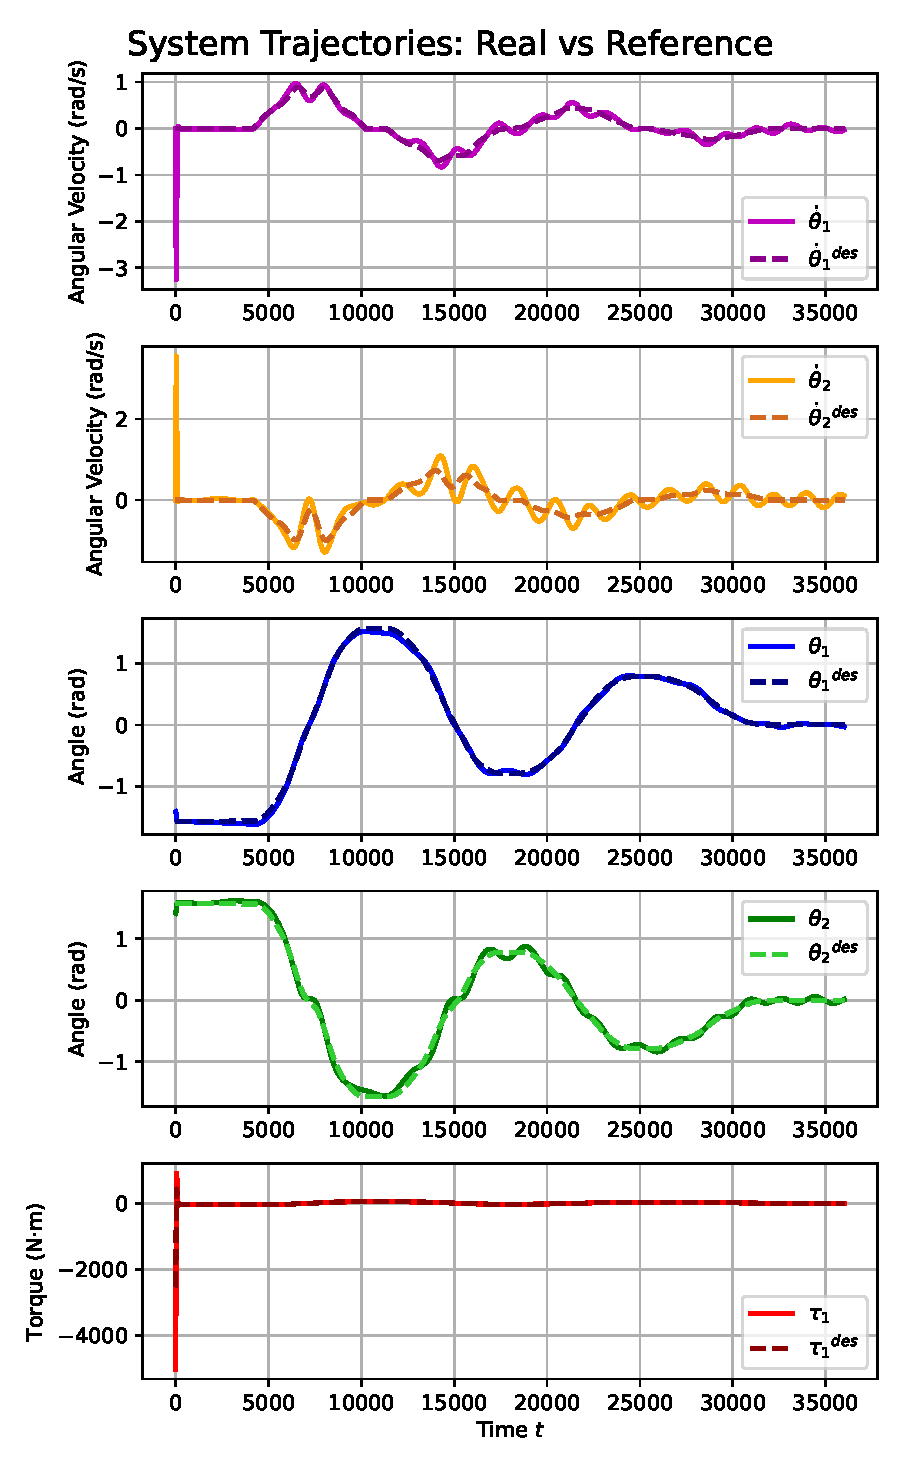
\includegraphics[width=1\linewidth]{img/3-task3/LQR3.pdf}
    \caption{Trajectories case 3}
    \label{fig:dtheta1-evolution}
\end{figure}

\begin{figure}[htb]
    \centering
    % First 3 images on the first page
    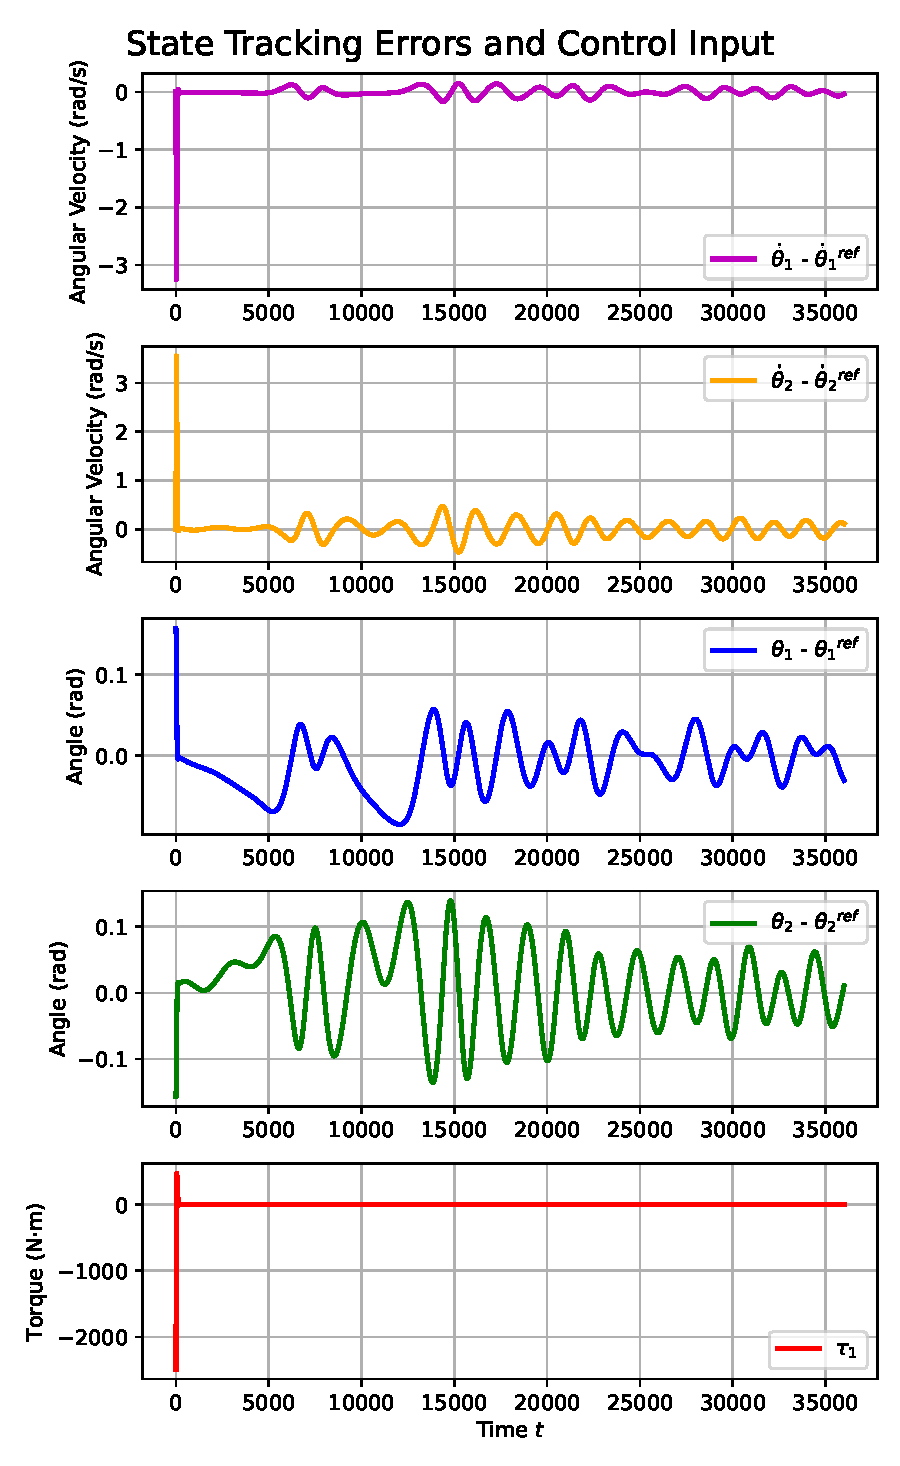
\includegraphics[width=1\linewidth]{img/3-task3/LQR3_errors.pdf}
    \caption{Tracking errors case 3}
    \label{fig:dtheta1-evolution}
\end{figure}
